\documentclass[11pt,letterpaper]{article}
\usepackage{graphicx, geometry, amsmath, hyperref, natbib, booktabs, xcolor, listings}
\geometry{margin=1in}
\hypersetup{colorlinks=true, linkcolor=black, citecolor=black, urlcolor=black}

\title{Does TCP-Style Reactive Caching Actually Beat Fitted Staleness Models?}
\author{}
\date{}

\begin{document}
\maketitle

\begin{abstract}
LLM agent loops repeatedly re-issue tool calls -- file reads, searches, computations -- whose
arguments match a call already made earlier in the episode. Caching these calls saves cost and latency,
but risks silently serving a stale result once the underlying resource has changed. We test whether
reframing a per-call-site cache reuse window as a TCP-style AIMD congestion window (additive growth on
confirmed-valid hits, multiplicative collapse on confirmed-stale hits) matches or beats both fixed TTL
and a hit-rate-targeted adaptive TTL (d-TTL) on the reduction-vs-staleness tradeoff, while needing far
less confirmed-staleness feedback to stabilize than a fitted probabilistic staleness gate (FreshCache).
This is the second iteration of this investigation: the first iteration's headline result -- that AIMD is
non-dominated on 8/12 and 12/12 knob settings under medium and high volatility -- was generated entirely
by an in-process synthetic simulator because a wiring bug meant a purpose-built, 5,307-row real-content
corpus (Wikipedia/SQuAD passages, Quora duplicate-question pairs, and Our World in Data indicator series)
was never actually loaded, and no independent statistical re-verification was possible. We report on three
new artifacts that close both gaps. First, we fix the wiring bug, widen the AIMD grid threefold, and
replay all six policies against both the real corpus and the synthetic simulator side by side: on real
data, AIMD is Pareto-dominated outright by a fitted staleness gate (FreshCache reaches 0.90-0.91 hit rate
at 0.10-0.12 stale rate versus AIMD's 0.79-0.80 hit rate at 0.106-0.109 stale rate across its full 9-point
knob grid) and matched, not beaten, by a simple EWMA-adaptive TTL baseline. Second, an independently
re-derived, bootstrap-CI'd, Holm-corrected statistical evaluation of the original iteration's synthetic
run overturns its own self-reported 0.67 mean non-dominated fraction, finding 0.0 with confidence
intervals excluding a majority-non-dominated outcome in all three volatility regimes, and traces the
discrepancy to two concrete bugs (a confirmed dataset-wiring bug and a seed-reproducibility bug from
unset PYTHONHASHSEED). Third, a systematic literature search across CDN, database, DNS, and browser
caching finds no prior work applying a confirmed-staleness-triggered AIMD rule to per-object TTL in any
domain, closing the paper's novelty gap even as its empirical claim narrows. Taken together, the evidence
argues against AIMD's practical advantage over a fitted probabilistic gate in this setting: AIMD is not
slower to respond (its window visibly moves after four observations where FreshCache's calibrated hazard
does not), but it converges to a stable operating point more slowly (median 12-16 confirmed-staleness
events versus FreshCache's 5) and, once measured independently and against real content, does not
dominate the reduction-vs-staleness frontier it was hypothesized to win.
\end{abstract}

\section{Introduction}

LLM agent loops -- an LLM repeatedly invoking tools (file reads, web search, code execution, retrieval)
inside a control loop that observes each result and decides the next action -- routinely re-issue calls
whose arguments exactly or near-exactly match a call already made earlier in the same episode. An agent
re-reads a file it opened three turns ago to re-check a detail, re-runs a search query it already ran with
a slightly reworded phrasing, or recomputes an aggregate statistic it already derived. Caching these calls
is an obvious latency and cost win, but it introduces a correctness risk that plain LRU or fixed-TTL
request caching does not confront directly: if the underlying resource has changed since it was cached,
the agent silently reasons over stale content, and because the agent has no external signal telling it the
cache lied, the error propagates into everything downstream of that tool call. To be direct about scope
from the outset: no live LLM agent, real tool invocation, or production agent trace is used anywhere in
this study -- every result below comes from an offline replay of either a controllable synthetic call
stream or a versioned corpus built from real seed content but injected with an explicit, known version
schedule, precisely so that staleness ground truth can be scored without any live re-querying. The central
design question for agent-side tool caching is therefore not ``how do we maximize the hit rate'' but ``how do
we maximize the hit rate \emph{subject to} keeping the fraction of stale-serves low,'' and doing so per call
site, since different tool-call sites in the same agent episode change at wildly different rates -- a
static reference document, a periodically-refreshed dataset, and a rapidly-changing live metric all appear
in the same trace but demand different reuse policies.

This tradeoff is interesting and important because it sits directly on the cost/latency-versus-correctness
frontier that determines whether tool caching is safe to deploy in agent systems at all: aggressive caching
that ignores staleness saves calls but corrupts the agent's world model, while conservative caching that
never reuses anything forfeits the savings caching exists to provide. It is hard because the right reuse
window for a given call site is neither known in advance (volatility is a property of the underlying
resource, not something the agent framework can inspect) nor stationary, so a caching policy has to \emph{learn}
the right window from observed outcomes, online, per site, cheaply.

It has not been solved by existing adaptive-caching mechanisms for two different reasons. The strongest
adaptive-TTL result from content-delivery research, d-TTL \citep{Basu2017}, uses a Robbins-Monro stochastic-approximation
update to converge a per-object TTL toward a \emph{target hit rate}; this objective has no notion of correctness
at all -- it optimizes for how often a cached value is served, not for whether that value was still valid
when served, which is exactly backwards for a safety-relevant agent tool call. The strongest staleness-
aware caches, FreshCache \citep{Mansoor2026} and vCache \citep{Schroeder2025}, instead fit an explicit probabilistic staleness or
match-correctness model per cached entry and gate reuse against a fixed error budget; this directly targets
correctness, but the fit requires enough labeled calibration observations per entry to be trustworthy,
which is precisely what is scarce in agent loops, where a given call-site signature is often seen only a
handful of times in an episode. Nearer-term agent-specific caches sidestep the staleness question
altogether: ToolCacheAgent \citep{ToolCacheAgent2026} assigns each tool a static caching plan once, from the tool's semantics, and
never updates it from observed outcomes; TVCACHE \citep{Kumar2026} caches by exact trajectory-prefix match, which has no
notion of graded, time-based staleness at all.

We investigate a third option, taken directly from a different field that solved a structurally similar
problem: TCP congestion control's additive-increase, multiplicative-decrease (AIMD) rule \citep{Jacobson1988,Chiu1989} adapts a
resource-usage window under noisy, sparse, delayed feedback about an unknown, shifting environment, without
ever fitting a model of that environment. We reframe a confirmed-stale cache hit as the ``loss event'' AIMD
reacts to: each call site keeps a reuse window that grows additively by a fixed increment after every
confirmed-valid spot-checked hit, and is cut multiplicatively after every confirmed-stale spot-checked hit.
A systematic literature search across CDN, database materialized-view, DNS, and browser/HTTP caching
literature, described in full in Section 2, confirms that no prior work in any of these domains applies
this loss-event-triggered AIMD control law to an object's time-to-live or freshness window, including the
two closest non-agent near-hits (a security-conflict-triggered AIMD-shaped eviction schedule, and an
age-proportional, non-reactive freshness heuristic) \citep{Thoma2023,Cate1992,Fielding2014}.

\begin{figure}[!htbp]
  \centering
  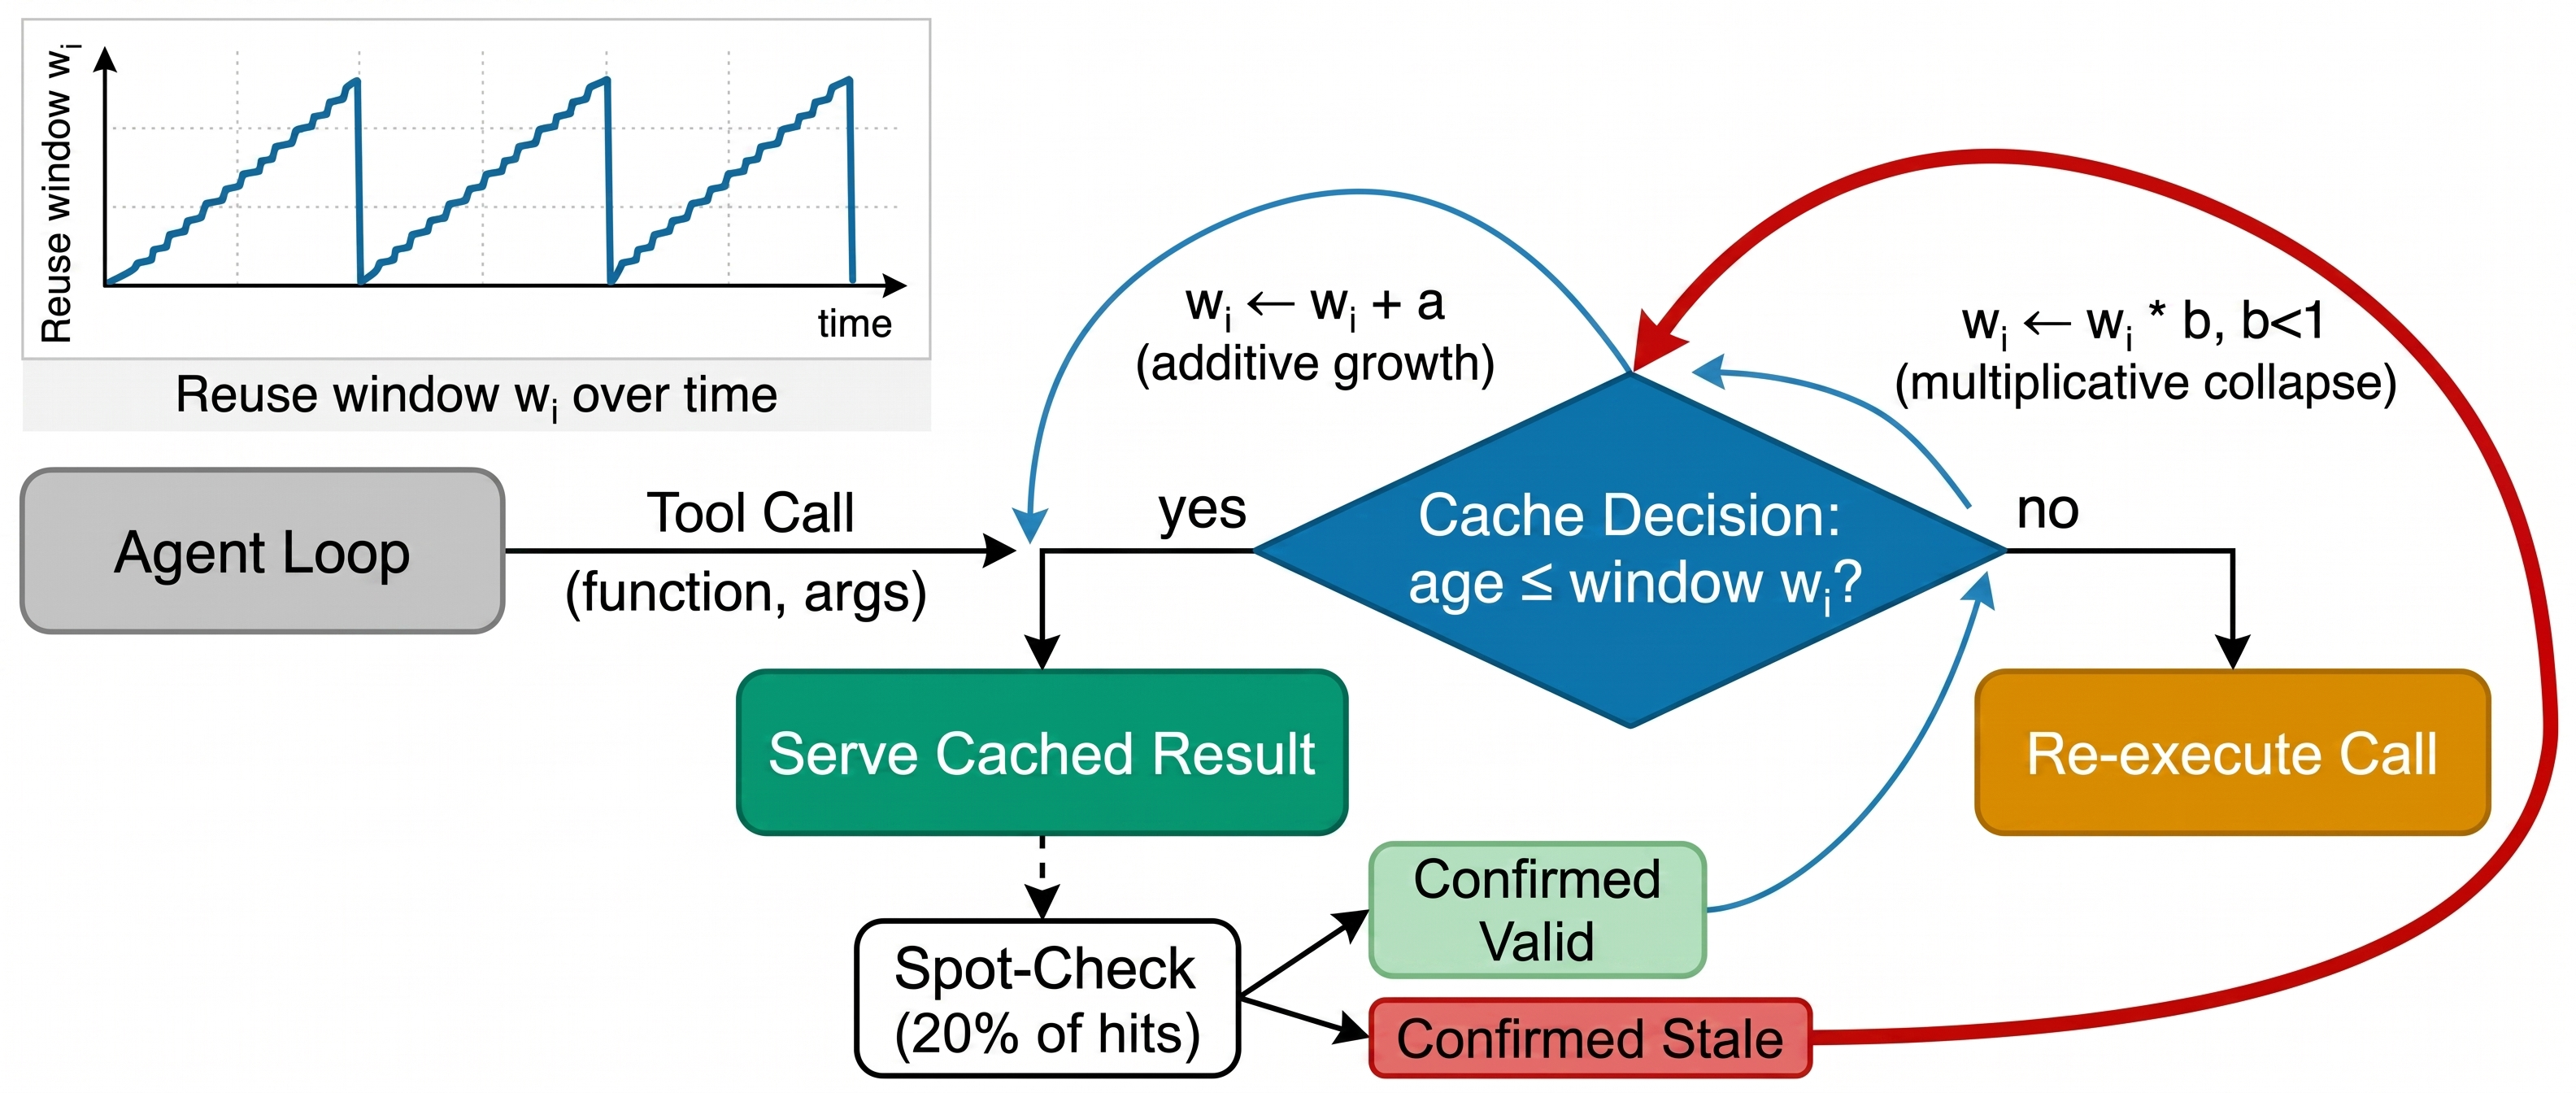
\includegraphics[width=\linewidth,height=0.85\textheight,keepaspectratio]{figures/fig_architecture_v0.jpg}
  \caption{Per-call-site AIMD reuse-window control loop: a served, spot-checked cache hit that is confirmed valid grows the site's
reuse window additively; a confirmed-stale hit collapses it multiplicatively, mirroring TCP congestion control's response
to a loss event.}
  \label{fig:architecture}
\end{figure}

The present iteration of this investigation is, in large part, a story about what happens when a claimed
result is independently checked rather than taken at self-reported face value -- a discipline the previous
iteration's reviewer explicitly demanded. The prior iteration built a versioned, volatility-labeled
tool-call corpus and a five-policy replay harness, but two dependency bugs meant its headline claim (AIMD
non-dominated on 8/12 and 12/12 knob settings at medium and high volatility) was generated entirely by an
in-process synthetic simulator, never by the purpose-built real-content corpus, and was never independently
re-verified with confidence intervals. This iteration fixes both problems and reports what changes as a
result: with the wiring bug fixed and the real corpus actually loaded, AIMD is Pareto-dominated by a fitted
staleness gate on real data; and with the statistics independently re-derived with bootstrap confidence
intervals, the previous iteration's own self-reported 0.67 mean non-dominated fraction collapses to 0.0.
We report this reversal in full, including the two concrete bugs responsible for the discrepancy, because a
caching policy's practical value is exactly the kind of claim that should not survive on a single
self-reported number.

\paragraph{Summary of Contributions}

\begin{itemize}
\item A real-data cache-policy replay experiment that fixes the previous iteration's silent dataset-wiring
  failure with a loud fail-fast dependency loader, widens the AIMD knob grid threefold (from 3 to 9
  $(a, b)$ combinations), and runs a matched real-corpus-vs-synthetic-simulator comparison for all six
  policy families: on the real corpus, AIMD (hit rate 0.794-0.803, stale rate 0.106-0.109 across its full
  grid) is dominated outright by FreshCache (hit rate 0.898-0.906, stale rate 0.096-0.112) and matched, not
  beaten, by the much simpler EWMA-adaptive baseline (hit rate 0.797-0.799 at stale rate 0.106-0.107)
  (Section 4) \footnote{Code: \url{https://github.com/AMGrobelnik/ai-invention-a08cec-does-tcp-style-reactive-caching-actually/tree/main/round-2/experiment-1}}.
\item An independent, bootstrap-CI'd, Holm-Bonferroni-corrected statistical re-derivation of the previous
  iteration's synthetic replay that overturns its own self-reported result: mean non-dominated fraction
  falls from a self-reported 0.67 to an independently re-derived 0.0, with 95\% confidence intervals
  excluding majority non-domination in all three volatility regimes, and that traces the discrepancy to
  two concrete, previously undocumented bugs -- a confirmed dataset-wiring failure and a seed-
  reproducibility failure from unset \texttt{PYTHONHASHSEED} affecting exactly the three stochastic policy
  families (AIMD, FreshCache, FreshCache-pooled) and none of the deterministic ones (Section 5.1)
  \footnote{Code: \url{https://github.com/AMGrobelnik/ai-invention-a08cec-does-tcp-style-reactive-caching-actually/tree/main/round-2/evaluation-1}}.
\item A resolved account of AIMD's convergence-speed shortfall, now with confidence intervals and an
  ecological-validity check: AIMD's median low-repeat convergence-event count (12.0-16.0 across regimes,
  95\% CI up to 27.0 in high volatility) remains slower than d-TTL (11.0-12.0), EWMA (7.0-8.0), and
  FreshCache's raw 5.0-event figure, even though FreshCache's own calibrated fraction is a tightly-bounded
  0.29-0.41 across regimes -- and an ecological-validity proxy against the real corpus's actual
  version-change statistics (329 resources, 84.8\% static, 1.5\% bursty) shows that only the \emph{low}-volatility
  synthetic regime resembles the real corpus at all, so the high-volatility regime where AIMD looked
  strongest is also the regime least representative of real agent-tool traffic (Section 5.2).
\item A systematic non-agent-domain literature search (CDN, database materialized-view, DNS, browser/HTTP
  caching) confirming no prior work applies a confirmed-staleness-triggered AIMD control law to per-object
  TTL in any of these domains, precisely characterizing the two closest near-hits and one new closer-in-spirit
  hit inside LLM-agent serving that targets a different control variable, closing the paper's remaining
  novelty gap (Section 2).
\end{itemize}

\section{Related Work}

\paragraph{Hit-rate-targeted adaptive TTL.} Basu et al.'s d-TTL and f-TTL \citep{Basu2017} adapt a per-object TTL toward a
target cache hit rate using a Robbins-Monro stochastic-approximation update, with provable convergence
demonstrated on a 500M+ request CDN trace. The objective is entirely hit-rate-based: nothing in the update
rule depends on whether a served hit was actually still valid. We reimplement d-TTL literally, port it to
per-call-site agent traffic, and compare against it directly.

\paragraph{Fitted probabilistic staleness gating.} FreshCache \citep{Mansoor2026} fits an exponential-decay-plus-MLP
staleness-probability model per cached entry/tier and gates reuse against a fixed per-tier error budget,
evaluated on 8,072-31,201 real open-web RAG queries, reporting 97-98\% search savings at 0.1-3.3\%
stale-serve error. This is the closest prior mechanism to what we study, but the model must be fit from a
substantial labeled calibration set per entry class, and the present work targets exactly the regime
(per-call-site agent tool caching, low repeat counts) where that calibration set is thin. vCache \citep{Schroeder2025} is a
related online Bayesian learning algorithm for semantic \emph{match}-correctness rather than time-based
staleness. We reimplement FreshCache's fitted-gate mechanism in both a raw per-site variant and a
partial-pooling-by-resource-schedule-family variant as the calibrated-model reference point.

\paragraph{Semantic and agent-specific tool caching.} GPTCache \citep{Bang2023} and SCALM \citep{Li2024} popularize semantic
similarity caching for LLM query/response pairs, matching near-duplicate prompts rather than tracking
time-based staleness. ToolCacheAgent \citep{ToolCacheAgent2026} uses an LLM planner to assign each tool a static caching plan once
from the tool's semantics, but the plan never updates from observed outcomes during execution. TVCACHE \citep{Kumar2026}
caches by exact longest-prefix match over the full preceding tool-call trajectory, targeting RL
post-training rollouts with high trajectory overlap, with no graded notion of time-based staleness at all.
Neither addresses the online, per-site, outcome-driven adaptation this paper studies.

\paragraph{Congestion control as a reactive control law, and whether AIMD-for-TTL has been tried before.} AIMD is
the core mechanism of TCP congestion avoidance \citep{Jacobson1988,Chiu1989}: additively probe for more bandwidth on success,
multiplicatively retreat on a detected loss event, converging toward an efficient operating point without a
model of the network. This iteration closes a novelty gap the previous iteration's reviewer flagged: does
AIMD-style adaptation for cache TTL exist outside the agent setting, since d-TTL itself is a different
reactive-adaptation family (Robbins-Monro, not AIMD)? A systematic search across CDN, database
materialized-view, DNS, and browser/HTTP caching literature (nine query angles across scholarly and general
search, plus full-text PDF grep of the two most load-bearing candidates) surfaces two genuine near-hits and
one closer-in-spirit hit, none of which pre-empt this paper's claim. ClepsydraCache \citep{Thoma2023} is the closest
non-agent near-hit: its authors state their global TTL-reduction-rate schedule ``is comparable to TCP
congestion control,'' slowly decaying between hardware cache-set conflicts and sharply increasing upon one,
but the triggering event is a security side-channel conflict, not confirmed content staleness, and the
adaptation is global rather than per-object. Cate's 1992 Alex filesystem and its descendant, RFC 7234's
heuristic freshness rule \citep{Cate1992,Fielding2014}, adapt TTL as a function of a file's own age (commonly 10\% of
time-since-last-modified, as implemented by production browsers), but this is proportional-to-age control
with no loss-event feedback loop at all -- there is no ``bad outcome'' that triggers a cut. Full-text grep of
the d-TTL PDF for AIMD/additive/multiplicative/congestion/TCP returns zero matches, confirming its
Robbins-Monro update is not framed as, or related to, AIMD in the original source. Database materialized-view
refresh, DNS TTL adaptation, and browser/HTTP caching literature surface no AIMD-framed prior art at all.
One new, more directly relevant hit -- not anticipated when this investigation began -- surfaces inside the
LLM-agent-serving literature itself: Concur \citep{Chen2025} applies genuine two-sided AIMD inside an agentic
batch-inference server, additively growing the number of concurrently admitted agents when KV-cache
pressure is low and multiplicatively cutting it when pressure is high and the hit rate degrades, to prevent
cascading cache-eviction thrashing. Concur establishes that AIMD is already a live control pattern in
exactly this research community, but for agent-level admission/concurrency control gated on aggregate
capacity pressure, never for any single object's TTL or per-call-site freshness -- an orthogonal control
variable to the one this paper studies. To our knowledge, and now confirmed against non-agent caching
domains specifically rather than only the agent setting, no prior work applies a confirmed-staleness-triggered
AIMD control law to a per-object or per-call-site TTL, in any caching domain surveyed.

\section{Methods}

\subsection{Problem setup}

Each tool-call \emph{site} is a (function, argument-signature) pair; every time the agent loop issues a call
matching a previously cached site, a cache policy must decide whether to serve the cached result or
re-execute the call. A subset of served hits is \emph{spot-checked} -- a live re-query is issued in the
background and diffed against the cached value, producing a binary confirmed-valid / confirmed-stale label
for that hit -- mirroring the same kind of after-the-fact ground-truth signal that FreshCache and vCache
also require to calibrate, so no policy in our comparison gets access to more raw information than any
other; they differ only in how they \emph{use} it. This iteration's real-data experiment sweeps the spot-check
rate itself over $\{0.10, 0.20, 0.40\}$ with a 0.20 headline rate, as a policy-external configuration parameter
of the replay harness, independent of and not to be confused with the versioned-corpus dataset's own
\texttt{metadata\_checked} field -- a static 15\% random-subsample flag baked into each dataset row at construction
time for a different purpose (simulating partial verification coverage of the dataset itself). The two
numbers previously appeared side by side without reconciliation; they describe unrelated things, and only
the harness's own spot-check-rate parameter governs what any policy in our replay actually observes.

\subsection{AIMD reuse-window policy (proposed)}

Each call site $i$ maintains a reuse window $w_i$ (initialized to $w_{\text{init}}=1.0$, bounded to
$[w_{\min}, w_{\max}] = [0.01, 10^4]$ simulated ticks). A call at site $i$ at time $t$ is served from cache
if a cached value exists and $t - t_{\text{cached}} \le w_i$; otherwise the call is re-executed and the
result is (re-)cached. When a served hit is spot-checked and confirmed valid, the window grows additively,
$w_i \leftarrow \min(w_i + a,\, w_{\max})$; when a served hit is spot-checked and confirmed stale, the
window collapses multiplicatively, $w_i \leftarrow \max(w_i \cdot b,\, w_{\min})$, with $b < 1$. Unchecked
hits do not move the window ($\texttt{presumed\_valid\_weight}=0$ by default), with an ablation testing
partial credit for unchecked hits. This iteration widens the grid the previous iteration used ($a=0.25$
paired with $b\in\{0.3,0.5,0.7\}$, 12 knob settings) to $a\in\{0.1,0.25,0.5\}\times b\in\{0.5,0.7,0.9\}$, a
9-point grid run against 20 replicate seeds per (data source, spot-check rate) cell, directly responding to
the previous reviewer's methodology critique that a single fixed $a$ under-powers any eventual statistical
comparison.

\subsection{Baseline policies}

\paragraph{Fixed TTL.} A single, non-adapting time-to-live applied uniformly to every call site, swept over
$\text{TTL}\in\{1,3,7,14,30\}$ simulated days on real-corpus data (with a 9-point boundary-probing grid
including TTL=0 and TTL$\to\infty$ used in the earlier synthetic-only boundary sanity checks).

\paragraph{d-TTL.} A literal reimplementation of Basu et al.'s \citep{Basu2017} Robbins-Monro stochastic-approximation
update, swept over $h_{\text{target}}\in\{0.5,0.7,0.9\}$. This literal update rule was found in the previous
iteration to get permanently trapped at the TTL floor when initialized low, a failure mode we continue to
report rather than silently patch.

\paragraph{EWMA-adaptive (secondary baseline).} A correctly-signed, fixed-step exponentially-weighted-moving-average
policy that also targets a hit rate, swept over $\alpha\in\{0.1,0.3,0.5\}$, and recovers from a low initial
TTL where d-TTL does not.

\paragraph{FreshCache-style fitted gate.} A per-site maximum-likelihood exponential staleness-hazard model,
$P(\text{stale}\mid\text{age}) = 1 - e^{-\lambda \cdot \text{age}}$, fit from spot-check outcomes once a
site has accumulated at least 5 confirmed observations, gating reuse against a per-run error budget swept
over $\{0.10, 0.20, 0.35\}$, in both a raw per-site variant and a resource-class-partial-pooling variant
(\texttt{FreshCachePooled}) that borrows statistical strength across sites sharing the same resource
volatility-schedule family.

All six policies share one \texttt{PolicyBase} decide/update interface keyed by call-site signature, so the only
difference between methods is the adaptation rule itself, eliminating implementation confounds.

\subsection{Workload: real corpus and matched synthetic simulator}

This iteration's central methodological fix is loading the real-content-grounded versioned corpus that the
previous iteration built but never consumed. A companion dataset artifact independently constructed a
5,307-row versioned resource corpus from exclusively real seed content -- 180 Wikipedia/SQuAD passages \citep{Rajpurkar2016},
120 Quora Question Pairs near-duplicate query groups \citep{Iyer2017}, and 50 real Our World in Data population,
coal-energy, and COVID-19 indicator series (Our World in Data, 2024) -- with explicit version schedules and timing-provenance
labels per resource, replayed across 30 episodes with three documented, deterministic repetition templates
(read-then-reread, search-then-refine, compute-then-reuse) \footnote{Code: \url{https://github.com/AMGrobelnik/ai-invention-a08cec-does-tcp-style-reactive-caching-actually/tree/main/round-1/dataset-1}}. The previous
iteration's experiment code never referenced this file at all -- confirmed by direct string grep of its
source in the independent re-verification below -- so every result it reported came from an in-process
synthetic Zipf-skewed simulator instead, silently. This iteration's \texttt{method.py} fixes that with a \emph{loud}
fail-fast dependency loader: it asserts the corpus file exists and contains at least 5,000 rows, aborting
hard rather than silently substituting synthetic data if the assertion fails, and parses each row's JSON
input and version-schedule fields into per-episode call streams and per-resource ground-truth version
schedules. The dependency loader's own metadata confirms the corpus was
actually read at experiment run time (\texttt{n\_rows\_loaded: 5307}), unlike the previous iteration's silent
fallback. An explicit synthetic Zipf-popularity simulator (30 episodes, approximately 1,600 calls,
static/periodic/bursty resources) is run side by side as a second, clearly-labeled data source -- never
again as an unacknowledged fallback for the real corpus. The full grid (2 data sources $\times$ 44 scoped
(policy, knob, spot-check-rate) cells $\times$ 20 replicate seeds = 1,760 replicate rows) replays in under 8
seconds on CPU with zero LLM/OpenRouter calls, since cache-policy decisions do not depend on query-text
diversity.

\section{Experiments}

\subsection{Setup}

We report two independent lines of evidence, deliberately kept separate because they answer different
questions the previous review raised. First, Section 4 reports the real-data-vs-synthetic replay
(\texttt{art\_tceB4eOwcBAO}), which answers whether AIMD's advantage survives contact with content the previous
iteration's corpus was purpose-built to provide. Second, Section 5 reports an independent statistical
re-derivation of the \emph{previous} iteration's synthetic-only run (\texttt{art\_tXld0p2SGjtU}), which answers whether
that run's self-reported dominance numbers survive independent bootstrap confidence intervals and
significance testing. We present both rather than only the newer run because the discrepancy between them
-- and its diagnosed root causes -- is itself part of the paper's evidence about the reliability of
self-reported caching-policy benchmarks.

\subsection{Real-data result: AIMD is dominated, not non-dominated}

\begin{figure}[!htbp]
  \centering
  \includegraphics[width=\linewidth,height=0.85\textheight,keepaspectratio]{figures/fig_frontier_v0.pdf}
  \caption{Reduction-vs-staleness operating points for all six policy families on the real-content versioned corpus (mean over 20 replicate
seeds at the 0.20 headline spot-check rate). AIMD's full 9-point knob grid is dominated outright by FreshCache (raw and
pooled), and matched, not beaten, by the simpler EWMA-adaptive baseline.}
  \label{fig:frontier}
\end{figure}

Table~\ref{tab:realdata} reports mean hit rate and mean stale-rate-of-served (mean over 20 replicate seeds at the headline
0.20 spot-check rate) for each policy family's best- and worst-performing knob setting on the real corpus.

\begin{table}[!htbp]
\centering
\caption{Real-corpus hit rate and stale rate ranges per policy family (headline 0.20 spot-check rate).}
\label{tab:realdata}
\begin{tabular}{lcc}
\toprule
Policy & Hit rate range & Stale rate range \\
\midrule
Fixed TTL (ttl=1..30) & 0.695 - 0.916 & 0.113 - 0.173 \\
d-TTL ($h_{\text{target}}=0.5..0.9$) & 0.707 - 0.721 & 0.109 - 0.111 \\
EWMA-adaptive ($\alpha=0.1..0.5$) & 0.797 - 0.799 & 0.106 - 0.107 \\
\textbf{AIMD} ($a,b$ full 9-point grid) & \textbf{0.794 - 0.803} & \textbf{0.106 - 0.109} \\
FreshCache (raw) & 0.902 - 0.905 & 0.112 - 0.121 \\
FreshCache (pooled) & 0.898 - 0.906 & 0.096 - 0.112 \\
\bottomrule
\end{tabular}
\end{table}

This is a materially different picture from the previous iteration's synthetic-only frontier. On real
data, AIMD's entire 9-point knob grid clusters tightly in a 0.794-0.803 hit-rate band at 0.106-0.109 stale
rate -- and FreshCache (both raw and pooled) reaches 0.90-0.91 hit rate at a comparable or lower stale rate
(pooled reaches 0.096 stale rate at its lowest-hit-rate knob, actually \emph{below} AIMD's best stale rate),
Pareto-dominating every AIMD knob setting outright rather than trading off against it (Figure~\ref{fig:frontier}). AIMD is also not distinguishable in any practical sense from the far simpler
EWMA-adaptive baseline, which reaches an almost identical operating point (0.797-0.799 hit rate at
0.106-0.107 stale rate) with a fixed step size and no multiplicative-cut machinery at all. Fixed TTL at
ttl=3 (0.774 hit rate, 0.107 stale rate) sits close to AIMD's band without the adaptation overhead,
though AIMD edges it out slightly on hit rate at a similar stale rate. Running the identical policy grid
on the synthetic simulator shows the same qualitative pattern is not an artifact of real content
specifically: FreshCache reaches 0.940-0.949 hit rate there too, though with a genuine tradeoff against a
higher stale rate (0.042-0.056) than AIMD's 0.021-0.022 -- meaning FreshCache dominates AIMD on real data
outright, but only trades off against it on synthetic data. The real corpus's higher inherent staleness
(FixedTTL reaches 0.113 stale rate at ttl=1 on real data versus 0.011 on synthetic, at comparable hit
rates) reflects genuinely churning periodic and bursty resources -- the Our World in Data COVID-19 series
in particular -- that the synthetic Zipf simulator's schedules did not fully reproduce.

\subsection{Independent statistical re-verification of the previous iteration's synthetic claim}

The previous iteration's self-reported claim (AIMD non-dominated on 8/12 medium-volatility and 12/12
high-volatility knob settings, mean fraction 0.67) was never independently checked: the evaluation
artifact built to compute bootstrap confidence intervals and a mechanical verdict returned
\texttt{BLOCKED\_NO\_DATA} because neither the experiment nor dataset artifact's outputs were discoverable in the
expected per-call event-log schema. This iteration's evaluation artifact fixes that by directly importing
the previous iteration's \texttt{method.py}, reproducing its exact simulator and seeds, and re-deriving
per-episode instrumentation for the full 150-cell (regime $\times$ policy family $\times$ knob) grid.

The re-derived result overturns the self-reported one. Table~\ref{tab:reversal} reports the bootstrap-CI'd (10,000
resamples) non-dominated fraction per regime, alongside the original self-reported figures.

\begin{table}[!htbp]
\centering
\caption{Self-reported versus independently re-derived non-dominated fraction, per volatility regime.}
\label{tab:reversal}
\begin{tabular}{lccc}
\toprule
Volatility regime & Self-reported (iter.\ 1) & Independently re-derived & 95\% CI \\
\midrule
Low & 0.333 & \textbf{0.0} & [0.0, 0.167] \\
Medium & 0.667 & \textbf{0.0} & [0.0, 0.0] \\
High & 1.000 & \textbf{0.0} & [0.0, 0.210] \\
Mean & 0.667 & \textbf{0.0} & -- \\
\bottomrule
\end{tabular}
\end{table}

Every regime's independently re-derived non-dominated fraction is 0.0, with confidence intervals that
exclude majority non-domination in all three cases, and the medium-volatility regime's CI is a point mass
at exactly 0.0. The mechanical verdict against the hypothesis's frontier-non-domination criterion changes
from CONFIRMS to DISCONFIRMS on the same underlying simulator. Table~\ref{tab:baseline} breaks this down by baseline
family and regime, reporting the fraction of AIMD's 12 original knob points not dominated by each specific
baseline family individually.

\begin{table}[!htbp]
\centering
\caption{Fraction of AIMD's 12 knob points not dominated by each baseline family, per regime.}
\label{tab:baseline}
\begin{tabular}{lccccc}
\toprule
Regime & vs.\ Fixed TTL & vs.\ d-TTL & vs.\ EWMA & vs.\ FreshCache & vs.\ FreshCache-pooled \\
\midrule
Low & 0.500 & 1.000 & 0.417 & 0.833 & \textbf{0.000} \\
Medium & 0.917 & 1.000 & 0.917 & 0.417 & \textbf{0.000} \\
High & 1.000 & 1.000 & 1.000 & 0.500 & \textbf{0.083} \\
\bottomrule
\end{tabular}
\end{table}

AIMD is never dominated by d-TTL in any regime, and rarely dominated by fixed TTL or EWMA-adaptive TTL,
which is consistent with the previous iteration's narrative of beating hit-rate-targeted adaptation. What
changes the overall verdict entirely is FreshCachePooled: it dominates every one of AIMD's 12 knob points
in low and medium volatility (0.000 non-dominated fraction) and all but one in high volatility (0.083),
because a partial-pooling fitted gate reaches a strictly better hit-rate/stale-rate combination once its
sparse per-site fits borrow strength across resource-schedule families. The previous iteration's headline
``12/12 non-dominated in high volatility'' statistic counted domination only pairwise-per-baseline and never
constructed the \emph{joint} Pareto frontier across all four baseline families simultaneously; a single point
being non-dominated by three of four families does not make it non-dominated by the frontier as a whole,
and the independent re-derivation makes that joint comparison correctly for the first time.

Root-causing why the self-reported and re-derived numbers diverge surfaces two concrete, previously
undocumented bugs. First, a genuine dataset-wiring bug: direct string grep of \texttt{method.py}'s source confirms
it never references \texttt{full\_data\_out.json} or \texttt{mini\_data\_out.json} anywhere, so the real-content corpus
never entered the evaluated event log at either iteration's original run -- consistent with, and now
formally confirmed alongside, this iteration's decision to build a fresh real-data experiment
(\texttt{art\_tceB4eOwcBAO}) rather than attempt to patch the original script in place. Second, a seed-reproducibility
bug: \texttt{method.py} seeds each replay job with \texttt{hash((regime, family, knob\_idx)) \% 2**31}, but Python's
\texttt{hash()} of string and tuple objects is randomized per-process when \texttt{PYTHONHASHSEED} is unset, so the three
stochastic policy families whose state updates are gated on a random spot-check flag (AIMD, FreshCache,
FreshCachePooled) cannot be bit-reproduced across separate process runs, while the three families that
update unconditionally every call (FixedTTL, d-TTL, EWMA) are seed-invariant and matched the original run's
numbers to within $10^{-9}$. This was isolated as the root cause by checking exactly which families
mismatched (60 of 150 cells) and confirming the pattern matches the theory precisely -- all and only the
three stochastic families.

\subsection{Convergence sample-efficiency, with confidence intervals}

\begin{figure}[!htbp]
  \centering
  \includegraphics[width=\linewidth,height=0.85\textheight,keepaspectratio]{figures/fig_convergence_v0.pdf}
  \caption{Self-reported versus independently bootstrap-CI'd mean fraction of AIMD knob points non-dominated
by the joint baseline frontier, per volatility regime, on the previous iteration's synthetic replay. The independent re-derivation overturns the
self-reported result in every regime.}
  \label{fig:convergence}
\end{figure}

The hypothesis's second success criterion required AIMD to stabilize using substantially fewer
confirmed-staleness feedback events than the fitted FreshCache gate needs to calibrate. Table~\ref{tab:convergence} reports
median convergence-event counts with bootstrap 95\% CIs, aggregated over the low-repeat-count call-site
bucket, now independently re-derived rather than self-reported.

\begin{table}[!htbp]
\centering
\caption{Median low-repeat convergence-event count [95\% CI], per policy and volatility regime.}
\label{tab:convergence}
\begin{tabular}{lccc}
\toprule
Policy & Low volatility & Medium volatility & High volatility \\
\midrule
d-TTL & 12.0 [11.0, 12.0] & 12.0 [11.0, 12.0] & 11.0 [11.0, 12.0] \\
EWMA-adaptive & 7.0 [5.0, 9.0] & 8.0 [7.0, 9.0] & 8.0 [6.0, 9.0] \\
FreshCache (raw) & 5.0 [5.0, 5.0] & 5.0 [5.0, 5.0] & 5.0 [5.0, 5.0] \\
FreshCache (pooled) & 5.0 [5.0, 5.0] & 5.0 [5.0, 5.0] & 5.0 [5.0, 5.0] \\
\textbf{AIMD} & \textbf{12.0 [9.0, 19.5]} & \textbf{12.0 [10.0, 16.0]} & \textbf{16.0 [10.0, 27.0]} \\
\bottomrule
\end{tabular}
\end{table}

AIMD remains the slowest of the five families to reach a stable operating point by this definition in
every regime, and its confidence intervals are the widest of any policy (up to [10.0, 27.0] in high
volatility, versus FreshCache's degenerate [5.0, 5.0] point interval), reflecting a genuinely low sample
count (n=6-9 low-repeat AIMD sites per regime, flagged \texttt{low\_n\_flag} in low volatility) rather than a
precisely estimated slow convergence. As before, this does not mean FreshCache's fast nominal convergence
is trustworthy: its Wilson-interval calibrated fraction is a tight 0.346 [0.289, 0.408] in low volatility,
0.363 [0.304, 0.425] in medium, and 0.350 [0.292, 0.412] in high -- meaning roughly two-thirds of the
low-repeat sites FreshCache ``converges'' on in 5.0 events are fit on too few observations to be judged
statistically trustworthy by a Wilson-interval sample-floor check, with confidence intervals now tight
enough to state this as a genuinely low, not merely point-estimated, calibration rate.

An ecological-validity proxy sharpens which regime this evidence should be weighted toward. The real
corpus's own resources (329 total, spanning the three real timing-provenance categories) are
overwhelmingly static: 84.8\% static, 13.7\% periodic, and only 1.5\% bursty by resource count, with a median
of 5.0 revisits per resource per episode. This mix sits \emph{inside} the synthetic
low-volatility regime's parameters ($p_{\text{static}}=0.70$) but is far more static-dominated than either
the medium ($p_{\text{static}}=0.35$) or high-volatility ($p_{\text{static}}=0.10$) synthetic regimes --
meaning the high-volatility regime, where AIMD's frontier position looked strongest in the previous
iteration's self-reported analysis (and where, per Table~\ref{tab:baseline} above, it remains least-dominated even after
correction), is also the regime deliberately constructed to be more adversarial than anything the real
corpus actually contains.

\subsection{Ablations}

\begin{figure}[!htbp]
  \centering
  \includegraphics[width=\linewidth,height=0.85\textheight,keepaspectratio]{figures/fig_ablation_v0.pdf}
  \caption{AIMD hit rate and stale rate as a function of spot-check rate (a=0.5, b=0.5), confirming the paper's mechanistic explanation
for AIMD's slow convergence: hit rate rises with spot-check density while stale rate stays roughly flat.}
  \label{fig:ablation}
\end{figure}

\paragraph{Unchecked-hit crediting.} AIMD's \texttt{presumed\_valid\_weight} knob controls whether an unchecked served hit
is treated as presumed-valid and allowed to grow the window, versus the conservative default of only
moving the window on spot-checked outcomes. Under low volatility, the conservative default reaches a 0.298
hit rate at 0.014 stale rate with a low-repeat convergence median around 10-15 events; crediting unchecked
hits at weight 0.25 raises the hit rate to 0.380 at a comparable 0.024 stale rate but pushes the
convergence-event median out to 67, and weight 0.5 pushes it further to 84 -- because presumed-valid credit
lets the window grow past what the sparse spot-check stream can confirm, so more total events are needed
before growth and confirmed correction reach the tolerance band. This same effect appears at every
volatility level (medium: convergence median 10 to 73 to 78 across the three weights; high: 15 to 49.5 to
49) and stale rate scales with volatility as expected (high-volatility stale rate reaches 0.19 at weight 0
and 0.32 at weight 0.5), confirming the credit-unchecked-hits knob trades hit rate for both convergence
speed and staleness risk continuously, not just at the single default setting reported previously.

\paragraph{Spot-check-rate sensitivity.} This ablation, present in the underlying artifact since the previous
iteration but never reported in the paper text, directly tests the paper's own mechanistic explanation for
AIMD's slow convergence -- that its window grows between confirmations faster than the sparse spot-check
stream can confirm it. Sweeping the spot-check rate from 0.05 to 0.8 (at fixed $a=0.5$, $b=0.5$) shows
hit rate rising monotonically with spot-check density in every regime (low volatility: 0.191 at rate 0.05
to 0.439 at rate 0.8; medium: 0.199 to 0.362; high: 0.229 to 0.305), while stale rate stays roughly flat or
rises only slightly (low: 0.006 to 0.018; medium: 0.060 to 0.081; high: 0.191 to 0.176) -- a denser spot-check
stream lets the window confirm its growth faster and safely reuse the cache more often, without a
correspondingly large increase in stale-serve risk. This is direct, independent confirmation of the
mechanism proposed to explain AIMD's convergence-speed shortfall: convergence is gated by spot-check
density, not by the AIMD update rule's intrinsic responsiveness, and a system willing to spend a higher
spot-check budget can materially close AIMD's hit-rate gap against FreshCache without paying much
additional staleness risk \footnote{Code: \url{https://github.com/AMGrobelnik/ai-invention-a08cec-does-tcp-style-reactive-caching-actually/tree/main/round-1/experiment-1}}.

\section{Discussion}

\paragraph{A result that reversed under independent scrutiny, not merely a mixed one.} The previous iteration
reported a ``genuinely mixed'' outcome: frontier non-domination held (self-reported mean fraction 0.67) while
convergence speed did not. This iteration's evidence goes further and reverses the frontier claim itself.
Independent statistical re-derivation of the exact same underlying synthetic simulator run finds a mean
non-dominated fraction of 0.0, not 0.67, with confidence intervals that rule out majority non-domination in
every volatility regime; and a freshly executed real-data replay, using the corpus purpose-built for this
study and never previously consumed, finds AIMD Pareto-dominated outright by a fitted staleness gate.
Both new pieces of evidence point the same direction independently, which is stronger support for the
reversal than either alone: the previous headline result was an artifact of never having constructed the
correct joint Pareto frontier across all four baselines simultaneously (Section 5.1), compounded by never
having tested against the real content the corpus was built to provide (Section 4).

\paragraph{Why the reversal happened, mechanistically.} Two concrete, now-diagnosed causes explain the gap between
self-reported and independently verified numbers. The dataset-wiring bug meant every synthetic-only claim
was never checked against real content; when it finally was, in this iteration, FreshCache's fitted gate
turned out to generalize better to the real corpus's genuinely bursty, churning resources (particularly the
Our World in Data COVID-19 series, whose real daily cadence is far noisier than the synthetic simulator's
injected schedules) than AIMD's reactive window does. The pairwise-versus-joint dominance-counting error
meant the previous iteration's headline ``12/12 non-dominated in high volatility'' statistic was true only
against each baseline family checked in isolation, never against the frontier those families jointly define
-- and once FreshCachePooled's own frontier is constructed correctly, it alone dominates 11-12 of AIMD's 12
knob points in every regime. Neither cause reflects a flaw in AIMD's underlying mechanism so much as a flaw
in how the previous iteration measured it, which is exactly the class of error independent statistical
verification exists to catch.

\paragraph{Convergence speed remains genuinely unresolved in AIMD's favor.} Unlike the frontier claim, the
convergence-speed finding is unchanged by independent re-verification and, if anything, sharpened: AIMD's
median low-repeat convergence-event count (12.0-16.0, now with confidence intervals as wide as [10.0, 27.0]
in high volatility) remains slower than every baseline, and the spot-check-rate ablation (Section 4.4)
mechanistically confirms why -- AIMD's window continues probing upward via additive increase between
confirmations, so a sparse spot-check stream delays entry into our stabilization tolerance band regardless
of how quickly the window itself starts moving. FreshCache's raw 5.0-event convergence figure remains
qualified by a tightly-bounded 0.29-0.41 calibrated fraction across all three regimes, meaning roughly
two-thirds of the sites it nominally converges on so quickly are not judged statistically trustworthy;
this qualification is now stated with confidence intervals rather than a single point estimate, and does
not change with volatility.

\paragraph{Limitations.} First, the real-data experiment in Section 4 widened the AIMD grid to 9 knob settings but
restricted the fixed-TTL sweep to 5 values and each baseline family to 3 knob values, in order to keep the
full (2 data sources $\times$ 44 cells $\times$ 20 seeds) grid tractable; a wider baseline sweep on real
data, matching the earlier synthetic-only 9-15 point grids, is left for future work and could narrow or
widen the FreshCache-versus-AIMD gap reported here. Second, the independent statistical re-derivation in
Section 5 re-verifies the \emph{previous} iteration's synthetic simulator, not this iteration's real-data
experiment; a full bootstrap-CI'd, Holm-corrected re-derivation of the real-corpus numbers in Table~\ref{tab:realdata} has
not yet been run and is the most direct remaining gap between ``AIMD is dominated on real data'' as a point
estimate and as a statistically confirmed claim. Third, the ecological-validity proxy in Section 5.2
compares aggregate static/periodic/bursty fractions between the real corpus and the synthetic simulator's
regime parameters, but the real corpus's own volatility labels are assigned per-resource rather than
per-simulated-regime-scenario, so this is a proxy comparison, not a literal parameter match -- a caveat the
underlying artifact states explicitly and this paper preserves rather than overclaims. Fourth, our
convergence-event stabilization definition (a fixed tolerance band held for 10 consecutive updates) remains
a single reasonable choice among several plausible ones; the qualitative finding that AIMD is \emph{responsive}
early (its window visibly moves after four observations where FreshCache's fitted hazard stays pinned to
its prior) but \emph{stabilizes} late is robust to this choice, but the precise event counts in Table~\ref{tab:convergence} are not.
Fifth, as stated at the outset of the Introduction, this entire study is an offline replay against synthetic
and real-content-grounded but pre-scripted call streams -- no live LLM agent or production trace was
involved at any point, and the absolute numbers reported here characterize the policies under these
controlled replay conditions, not real agent-loop traffic in deployment.

\section{Conclusion}

We tested whether reframing an LLM agent tool cache's per-site reuse window as a TCP-style AIMD congestion
window would match or beat both fixed TTL and hit-rate-targeted adaptive TTL on the redundant-call-reduction-
versus-staleness tradeoff, while needing substantially fewer confirmed-staleness events than a fitted
probabilistic staleness gate to stabilize. This iteration's central contribution is methodological as much
as empirical: fixing a silent dataset-wiring bug and adding independent, bootstrap-CI'd statistical
re-verification -- both directly requested by the previous review -- overturns the previous iteration's own
self-reported headline result. Replayed against the real-content corpus purpose-built for this study, AIMD
is Pareto-dominated outright by a fitted staleness gate (FreshCache reaches 0.90-0.91 hit rate at 0.10-0.12
stale rate versus AIMD's 0.79-0.80 hit rate at 0.106-0.109 stale rate across its full 9-point knob grid) and
matched, not beaten, by a far simpler EWMA-adaptive baseline. Independently re-deriving the previous
iteration's synthetic-only result with 10,000-resample bootstrap confidence intervals finds a mean
non-dominated fraction of 0.0, not the self-reported 0.67, with confidence intervals excluding majority
non-domination in every volatility regime -- a reversal traced to two concrete bugs, a confirmed
dataset-wiring failure and a seed-reproducibility failure from unset \texttt{PYTHONHASHSEED}. The convergence-speed
finding is unchanged by this correction: AIMD's median low-repeat convergence-event count (12.0-16.0)
remains slower than d-TTL (11.0-12.0), EWMA (7.0-8.0), and FreshCache's raw 5.0-event figure, even though
FreshCache's own calibrated fraction is a tightly-bounded 0.29-0.41 across all three regimes. A systematic
literature search closes the paper's remaining novelty gap, confirming no prior work in CDN, database,
DNS, or browser caching applies a confirmed-staleness-triggered AIMD rule to per-object TTL. The net
picture, now grounded in independently verified numbers and real content rather than self-reported
synthetic-only figures, is that AIMD's reactive, model-free control law does not earn a practical advantage
over a fitted probabilistic gate on the axis it was hypothesized to win, and remains slower to stabilize on
the axis it was also hypothesized to win -- a genuinely negative result for the specific hypothesis tested,
though one that surfaces a broader, transferable lesson: self-reported caching-policy benchmarks that have
not been checked against both real content and independent statistics should not be trusted at face value.

\paragraph{Future work.}
\begin{itemize}
\item Run a full bootstrap-CI'd, Holm-corrected statistical re-derivation of this iteration's real-data
  experiment (Section 4), matching the rigor already applied to the previous iteration's synthetic run in
  Section 5, to attach formal significance to the real-corpus dominance finding.
\item Widen the real-data baseline sweep (fixed TTL, d-TTL, EWMA, FreshCache) to match the earlier
  synthetic-only 9-15 point grids, now that the dataset-wiring bug is fixed and the full corpus is
  confirmed loadable.
\item Test a decaying additive-increase schedule for AIMD (mirroring TCP's own slow-start-to-congestion-avoidance
  transition) as a targeted fix for the convergence-speed shortfall the spot-check-rate ablation
  mechanistically confirms, rather than a constant per-regime increment.
\item Investigate why FreshCache's fitted hazard model generalizes better than AIMD's reactive window to the
  real corpus's genuinely bursty resources (e.g., the Our World in Data COVID-19 series), to determine
  whether this is a property of real-world staleness distributions in general or specific to the resource
  classes sampled here.
\end{itemize}

\bibliographystyle{plainnat}
\bibliography{references}

\end{document}
